
\tcbset{enobox/.append style={unbreakable}}
\Needspace{8\baselineskip}\subsection{Le dimensionnement du panneau}

\subsubsection*{Ce que je cherche et ce que je suppose}

Je pars de l'hypothèse que je n'ai pas encore de panneau. Je connais le besoin de la tour : $E_j = \qty{226,7}{Wh/j}$ (partie 5.3). Je cherche la puissance crête $P_c$, en watts-crête, qu'il faut pour couvrir ce besoin pendant le pire mois, puis je vérifie que le panneau que j'ai, le TE1250 de \qty{120}{Wc}, convient. Il me faut pour cela trois choses : l'énergie que le soleil apporte à Moorea pendant le pire mois, la part de cette énergie qui arrive vraiment dans les batteries (les pertes), et la formule qui relie ces grandeurs à la puissance crête. Je commence par l'ensoleillement.

\subsubsection*{L'ensoleillement à Moorea et le pire mois}

Pour l'ensoleillement, je prends les données de Solargis publiées par la Banque mondiale, moyennées sur les années 1999 à 2018. La grandeur utile est l'irradiation globale horizontale, notée GHI : c'est l'énergie solaire reçue par un mètre carré horizontal, en kWh/m$^2$. Les cartes ci-dessous donnent sa moyenne par jour, et le potentiel de production d'un panneau (PVOUT). Moorea est entourée en rouge.

\begin{figure}[H]
\centering
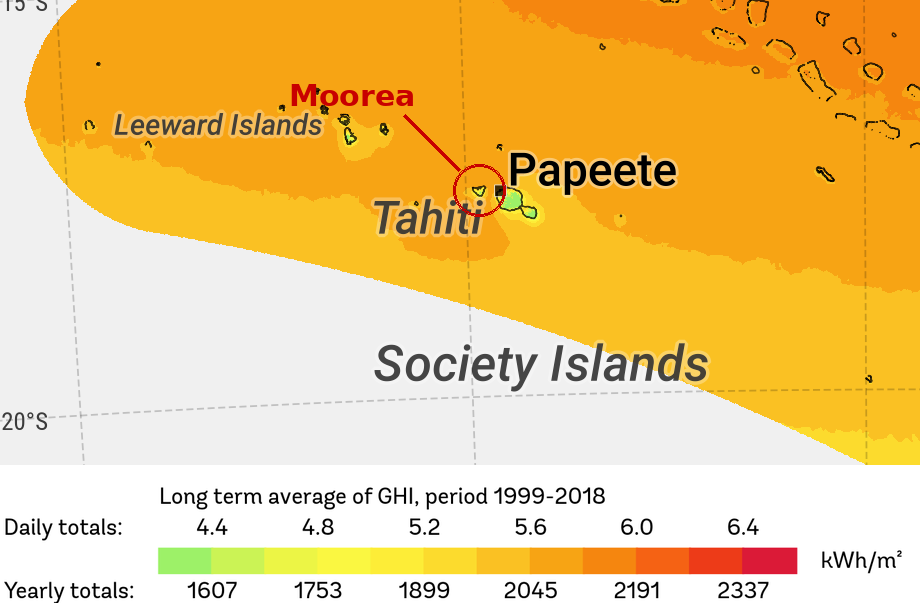
\includegraphics[width=0.86\textwidth]{img/solargis_ghi.png}
\caption{Irradiation globale horizontale (GHI), moyenne journalière sur 1999 à 2018, en Polynésie française (zone des îles de la Société). \copyright\ 2019 The World Bank, source : Global Solar Atlas 2.0, données Solargis. Le cercle rouge et le nom de Moorea ont été ajoutés.}
\end{figure}

Sur cette carte, les points de Moorea se répartissent entre les tranches de \num{4,4} à \qty{5,2}{kWh/m^2/j}, plus bas que l'océan autour (plus de \qty{5,4}{kWh/m^2/j}). Une carte ne donne qu'une moyenne sur l'année : elle ne dit pas quel mois est le plus sombre. Pour cela, je prends les moyennes mensuelles du Global Solar Atlas, qui repose sur les mêmes données Solargis, au point de Moorea (\qty{17,54}{\degree} sud, \qty{149,83}{\degree} ouest). Ces valeurs sont à valider avec mon tuteur.

\begin{figure}[H]
\centering
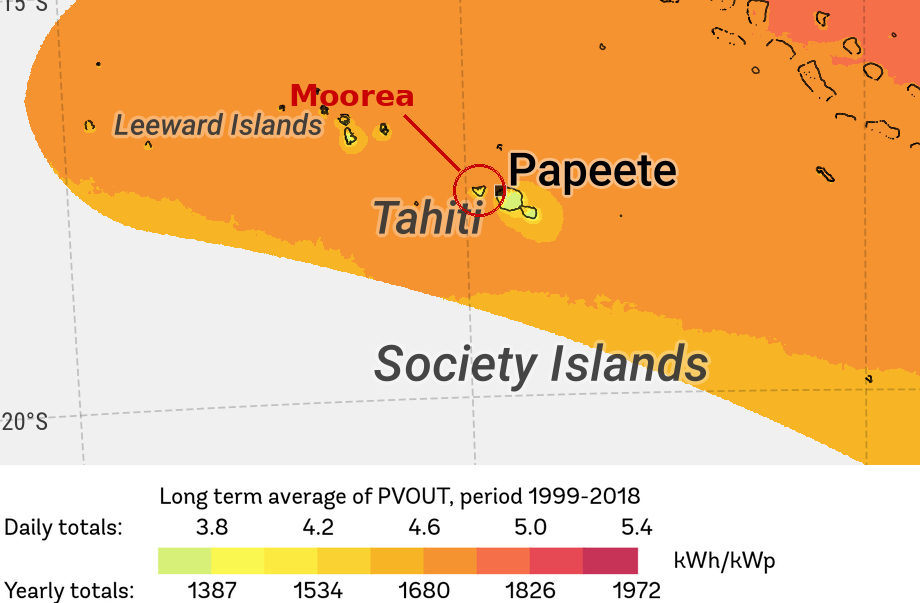
\includegraphics[width=0.86\textwidth]{img/solargis_pvout.png}
\caption{Potentiel de production photovoltaïque (PVOUT), moyenne journalière sur 1999 à 2018, en kWh par kWc. \copyright\ 2019 The World Bank, source : Global Solar Atlas 2.0, données Solargis. Le cercle rouge et le nom de Moorea ont été ajoutés.}
\end{figure}

La carte du PVOUT sert seulement de contrôle : elle suppose un panneau incliné de façon optimale et ses propres pertes, alors que je détaille moi-même chaque perte plus bas. Je ne m'en sers donc pas pour le calcul.

\naturecalc[22]{théorie (formule démontrée) appliquée à des données de Solargis ; rien de mesuré}
\begin{demonstration}[le pire mois d'ensoleillement]
\resultat{H_{pire} = \dfrac{G_{juin}}{N_{juin}} = \dfrac{\qty{108,21}{kWh/m^2}}{\qty{30}{j}} \approx \qty{3,607}{kWh/m^2/j}}
Je note $G_m$ l'irradiation reçue pendant le mois $m$, en kWh/m$^2$ par mois (donnée de Solargis), $N_m$ le nombre de jours de ce mois, et $H_m$ l'irradiation journalière moyenne du mois, en kWh/m$^2$/j. Le mois reçoit $G_m$ répartie sur $N_m$ jours, donc :
\begin{align*}
H_m &= \frac{G_m}{N_m}
\end{align*}
Le pire mois est celui où $H_m$ est le plus petit. Je calcule $H_m$ pour les douze mois dans le tableau ; le plus petit est juin :
\begin{align*}
H_{juin} &= \frac{\qty{108,21}{kWh/m^2}}{\qty{30}{j}}\\
H_{juin} &\approx \qty{3,607}{kWh/m^2/j}
\end{align*}
La moyenne sur l'année vaut $\qty{1731,45}{kWh/m^2}/\qty{365}{j} \approx \qty{4,74}{kWh/m^2/j}$ : le pire mois reçoit environ $\num{3,607}/\num{4,74} \approx 76\,\%$ de la moyenne.
\end{demonstration}

\begin{table}[H]
\centering
\small
\begin{tabular}{|l|c|c|c|}
\hline
\textbf{Mois} & \textbf{$G_m$ (kWh/m$^2$/mois)} & \textbf{$N_m$ (j)} & \textbf{$H_m$ (kWh/m$^2$/j)} \\
\hline
Janvier & 167,06 & 31 & 5,39 \\
\hline
Février & 153,28 & 28 & 5,47 \\
\hline
Mars & 164,42 & 31 & 5,30 \\
\hline
Avril & 136,11 & 30 & 4,54 \\
\hline
Mai & 122,48 & 31 & 3,95 \\
\hline
\textbf{Juin} & \textbf{108,21} & \textbf{30} & \textbf{3,61} \\
\hline
Juillet & 116,90 & 31 & 3,77 \\
\hline
Août & 134,17 & 31 & 4,33 \\
\hline
Septembre & 143,79 & 30 & 4,79 \\
\hline
Octobre & 158,01 & 31 & 5,10 \\
\hline
Novembre & 160,17 & 30 & 5,34 \\
\hline
Décembre & 166,84 & 31 & 5,38 \\
\hline
\end{tabular}
\caption{Irradiation globale horizontale à Moorea, moyennes 1999 à 2018 (Global Solar Atlas, données Solargis). La pire période est mai à juillet, et le pire mois est juin.}
\end{table}

La pire période est l'hiver austral, de mai à juillet, et le pire mois est juin. Le même site donne aussi l'irradiation sur un plan incliné de \qty{17}{\degree}, l'inclinaison optimale : \qty{129,24}{kWh/m^2} en juin, soit \qty{4,31}{kWh/m^2/j} ou \qty{19}{\percent} de plus que le plan horizontal. Mon panneau est incliné, mais son angle n'est pas fixé : je prends donc le plan horizontal pour dimensionner, et ce gain éventuel reste une marge en plus.

\subsubsection*{Le panneau que j'ai et ses données}

Je pars des données de l'étiquette du TE1250, dans les conditions standard (STC : \qty{1000}{W/m^2} et \qty{25}{\celsius}).

\begin{table}[H]
\centering
\small
\begin{tabular}{|l|c|c|}
\hline
\textbf{Grandeur (conditions STC)} & \textbf{Symbole} & \textbf{Valeur} \\
\hline
Puissance crête & $P_c$ & \qty{120}{Wc} \\
\hline
Puissance minimale garantie & $P_{\min}$ & \qty{117,5}{W} \\
\hline
Tension au point de puissance maximale & $V_{mp}$ & \qty{17,6}{V} \\
\hline
Courant au point de puissance maximale & $I_{mp}$ & \qty{6,8}{A} \\
\hline
Courant de court-circuit & $I_{sc}$ & \qty{7,3}{A} \\
\hline
Tension de circuit ouvert & $V_{oc}$ & \qty{22,0}{V} \\
\hline
Calibre maximal du fusible série & & \qty{10}{A} \\
\hline
\end{tabular}
\caption{Données d'étiquette du TE1250.}
\end{table}

Les coefficients de température du TE1250 ne figurent pas sur l'étiquette : je prends ceux du SLP055 (même technologie, 36 cellules), soit $\beta_V = -\qty{80}{mV/\celsius}$ pour la tension, $\gamma_P = -\qty{0,5}{\percent/\celsius}$ pour la puissance et une NOCT de \qty{47}{\celsius}. Je suppose une température d'air de \qty{27}{\celsius} en milieu de journée du pire mois (hypothèse).

\Needspace{30\baselineskip}\subsubsection*{La température des cellules}

\naturecalc[26]{théorie (formule démontrée, valeurs de fiches techniques et hypothèses ; rien de mesuré)}
\begin{demonstration}[température de cellule à partir de la NOCT]
\resultat{T_c = T_a + \dfrac{\mathrm{NOCT} - \qty{20}{\celsius}}{\qty{800}{W/m^2}}\, G \approx \qty{54}{\celsius}}
Je note $T_a$ la température de l'air, en °C, $T_c$ celle de la cellule, en °C, $G$ l'éclairement, en W/m$^2$, $\alpha$ la part de la lumière absorbée (sans unité) et $h$ le coefficient d'échange avec l'air, en W/(m$^2\cdot$K). La cellule reçoit une puissance proportionnelle à l'éclairement et la cède à l'air par convection et rayonnement, de façon à peu près proportionnelle à l'écart de température. En régime établi, puissance reçue égale puissance cédée :
\begin{align*}
\alpha\, G &= h\,(T_c - T_a)\\
T_c - T_a &= \frac{\alpha}{h}\, G = K\, G
\end{align*}
La NOCT est la température atteinte sous $G = \qty{800}{W/m^2}$ avec $T_a = \qty{20}{\celsius}$ (donnée de la fiche : \qty{47}{\celsius}) :
\begin{align*}
\mathrm{NOCT} - \qty{20}{\celsius} &= K \times \qty{800}{W/m^2}\\
K &= \frac{\mathrm{NOCT} - \qty{20}{\celsius}}{\qty{800}{W/m^2}}\\
T_c &= T_a + \frac{\mathrm{NOCT} - \qty{20}{\celsius}}{\qty{800}{W/m^2}}\, G
\end{align*}
Application, avec $T_a = \qty{27}{\celsius}$ et $G = \qty{800}{W/m^2}$ en milieu de journée du pire mois :
\begin{align*}
T_c &= \qty{27}{\celsius} + \frac{\qty{47}{\celsius} - \qty{20}{\celsius}}{\qty{800}{W/m^2}} \times \qty{800}{W/m^2}\\
T_c &= \qty{27}{\celsius} + \qty{27}{\celsius}\\
T_c &= \qty{54}{\celsius}
\end{align*}
\end{demonstration}

\Needspace{12\baselineskip}\subsubsection*{La puissance du panneau selon la température}

Je calcule directement sur le panneau entier, sans passer par un modèle de cellule. La figure donne les caractéristiques courant-tension et puissance-tension du TE1250, reprises de mon étude électrique de départ, sous \qty{1000}{W/m^2}, à quatre températures de cellule. Les températures de \qty{25}{\celsius} (conditions standard), \qty{47}{\celsius} (NOCT) et \qty{75}{\celsius} (cas extrême) encadrent la température de \qty{54}{\celsius} calculée plus haut.

\begin{figure}[H]
\centering
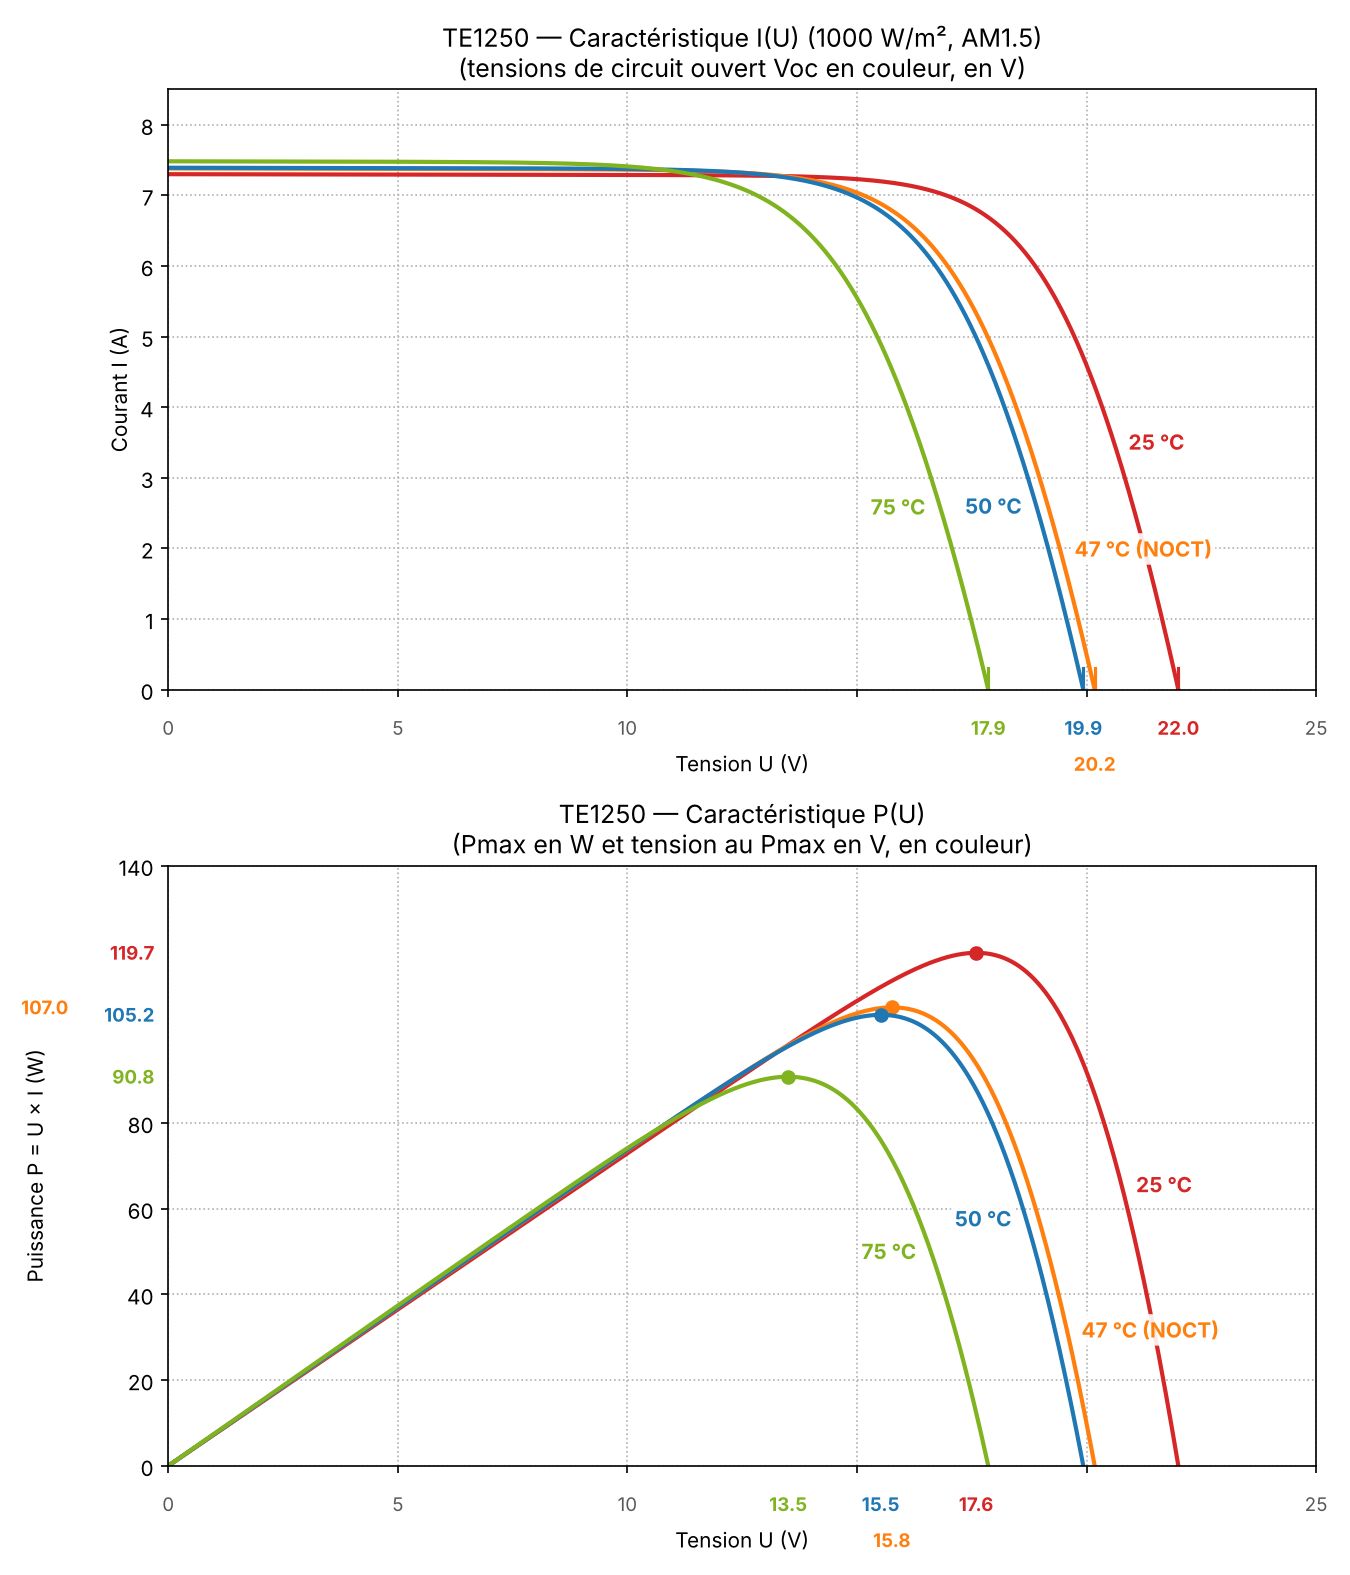
\includegraphics[width=0.62\textwidth]{img/elec/te1250_etude.png}
\caption{Caractéristiques $I(U)$ et $P(U)$ du TE1250 sous \qty{1000}{W/m^2}, reprises de mon étude électrique de départ.}
\end{figure}

\naturecalc[30]{théorie (formule démontrée, valeurs de fiches techniques et hypothèses ; rien de mesuré)}
\begin{demonstration}[puissance et tension du panneau selon la température]
\resultat{P_{\max}(T_c) = P_c\,[1 + \gamma_P\,(T_c - \qty{25}{\celsius})] \qquad k_T = 0{,}855}
Je note $T_c$ la température des cellules, en °C, $P_{\max}(T_c)$ la puissance maximale du panneau à cette température, en watts, et $\gamma_P$ le coefficient de température de la puissance, en 1/°C. Par définition, $\gamma_P$ est la variation relative de puissance par degré :
\begin{align*}
\gamma_P &= \frac{1}{P_c}\,\frac{\mathrm{d}P_{\max}}{\mathrm{d}T_c}
\end{align*}
La fiche donne $\gamma_P$ constant sur la plage de 25 à \qty{75}{\celsius}. La dérivée vaut donc $P_c\,\gamma_P$, constante : la puissance est une fonction affine de $T_c$. Je l'intègre entre \qty{25}{\celsius}, où elle vaut $P_c$, et $T_c$ :
\begin{align*}
P_{\max}(T_c) - P_c &= P_c\,\gamma_P\,(T_c - \qty{25}{\celsius})\\
P_{\max}(T_c) &= P_c\,[1 + \gamma_P\,(T_c - \qty{25}{\celsius})]
\end{align*}
Le facteur de température $k_T$ (sans unité) est le rapport $P_{\max}(T_c)/P_c$. Avec $\gamma_P = -\qty{0,005}{/\celsius}$ et $T_c = \qty{54}{\celsius}$ :
\begin{align*}
k_T &= 1 + \gamma_P\,(T_c - \qty{25}{\celsius})\\
k_T &= 1 - \qty{0,005}{/\celsius} \times (\qty{54}{\celsius} - \qty{25}{\celsius})\\
k_T &= 0{,}855
\end{align*}
La tension au point de puissance maximale se calcule de la même façon avec $\beta_V$, la variation de tension par degré, en V/°C :
\begin{align*}
V_{mp}(T_c) &= V_{mp} + \beta_V\,(T_c - \qty{25}{\celsius})
\end{align*}
À \qty{75}{\celsius} :
\begin{align*}
V_{mp}(\qty{75}{\celsius}) &= \qty{17,6}{V} - \qty{0,080}{V/\celsius} \times (\qty{75}{\celsius} - \qty{25}{\celsius})\\
V_{mp}(\qty{75}{\celsius}) &= \qty{13,6}{V}
\end{align*}
\end{demonstration}

Le tableau compare ce calcul direct aux valeurs lues sur les courbes de mon étude. À \qty{54}{\celsius}, la température n'est pas tracée : je lis la valeur par interpolation linéaire entre les courbes de \qty{50}{\celsius} et \qty{75}{\celsius}, par exemple $\qty{105,2}{W} + (\qty{90,8}{W} - \qty{105,2}{W}) \times (54 - 50)/(75 - 50) \approx \qty{102,9}{W}$.

\begin{table}[H]
\centering
\small
\begin{tabular}{|c|c|c|c|c|c|}
\hline
\textbf{$T_c$} & \textbf{$P_{\max}$ calcul (W)} & \textbf{$P_{\max}$ courbes (W)} & \textbf{Écart} & \textbf{$V_{mp}$ calcul (V)} & \textbf{$V_{mp}$ courbes (V)} \\
\hline
\qty{25}{\celsius} & 120,0 & 119,7 & $+$0,3\,\% & 17,6 & 17,6 \\
\hline
\qty{47}{\celsius} & 106,8 & 107,0 & $-$0,2\,\% & 15,8 & 15,8 \\
\hline
\qty{50}{\celsius} & 105,0 & 105,2 & $-$0,2\,\% & 15,6 & 15,5 \\
\hline
\qty{54}{\celsius} & 102,6 & 102,9 (interpolé) & $-$0,3\,\% & 15,3 & 15,2 (interpolé) \\
\hline
\qty{75}{\celsius} & 90,0 & 90,8 & $-$0,9\,\% & 13,6 & 13,5 \\
\hline
\end{tabular}
\caption{Calcul direct sur le panneau entier et valeurs de mon étude électrique de départ.}
\end{table}

Le calcul direct reste à moins de \qty{1}{\percent} des courbes : il me suffit pour dimensionner. Même à \qty{75}{\celsius}, $V_{mp} = \qty{13,6}{V}$ reste au-dessus de la tension de charge d'une batterie \qty{12}{V} vide : le régulateur MPPT\ix{19} peut toujours charger. C'est la principale raison d'utiliser un régulateur MPPT\ix{19} plutôt qu'une simple liaison directe.

\Needspace{36\baselineskip}\subsubsection*{L'énergie produite et la puissance crête nécessaire}

\naturecalc[30]{théorie (formule démontrée, valeurs de fiches techniques et hypothèses ; rien de mesuré)}
\begin{demonstration}[énergie produite à partir de l'irradiation journalière]
\resultat{E_{prod} = P_c\,\dfrac{H}{G_{STC}}\; k_T\, k_{tol}\, k_s\, k_{MPPT\ix{19}}\, k_{câbles}\, k_{bat}}
Je note $G_{STC} = \qty{1000}{W/m^2}$ l'éclairement des conditions standard, $G(t)$ l'éclairement à l'instant $t$, $H$ l'irradiation journalière, en Wh/m$^2$/j, et $E_{th}$ l'énergie théorique sans perte, en Wh/j. La puissance d'un panneau est proportionnelle à l'éclairement ; à $G_{STC}$ elle vaut $P_c$ :
\begin{align*}
P(t) &= P_c\,\frac{G(t)}{G_{STC}}
\end{align*}
J'intègre sur la journée :
\begin{align*}
E_{th} &= \int_{jour} P(t)\,\mathrm{d}t\\
E_{th} &= \frac{P_c}{G_{STC}} \int_{jour} G(t)\,\mathrm{d}t
\end{align*}
L'intégrale de l'éclairement sur la journée est l'irradiation journalière $H$ :
\begin{align*}
E_{th} &= P_c\,\frac{H}{G_{STC}}
\end{align*}
Le rapport $H/G_{STC}$ est un nombre d'heures, appelé heures équivalentes de plein soleil. Les pertes réelles se multiplient, chacune s'appliquant à ce qui reste après la précédente :
\begin{align*}
E_{prod} &= E_{th}\; k_T\; k_{tol}\; k_s\; k_{MPPT}\; k_{câbles}\; k_{bat}
\end{align*}
\end{demonstration}

Les facteurs retenus sont les suivants. Le facteur $k_T = 0{,}855$ vient de la température des cellules (calcul précédent). Le facteur $k_{tol} = 117{,}5/120 = 0{,}9792$ tient compte de la tolérance de fabrication (puissance minimale garantie de l'étiquette). Le facteur $k_s = 0{,}95$ tient compte des salissures, du sel marin, de la poussière et d'une orientation imparfaite. Le facteur $k_{MPPT} = 0{,}95$ est le rendement du régulateur (la fiche annonce jusqu'à \qty{97}{\percent}). Le facteur $k_{câbles} = 0{,}98$ tient compte des chutes de tension dans les câbles (partie 5.7). Le facteur $k_{bat}$ est le rendement énergétique de la charge puis de la décharge de la batterie : $0{,}95$ en LiFePO4 et $0{,}85$ en plomb AGM. Il est appliqué à toute l'énergie, alors qu'une partie est consommée directement le jour : c'est prudent. Le produit de tous ces facteurs est le rapport de performance $PR$ (sans unité).

\naturecalc[34]{théorie (formule démontrée, valeurs de fiches techniques et hypothèses ; rien de mesuré)}
\begin{demonstration}[puissance crête nécessaire]
\resultat{P_{c,\min} = \dfrac{E_j\,G_{STC}}{H\,PR} \approx \qty{99,9}{Wc}\ \text{(AGM)}\quad\text{ou}\quad \qty{89,3}{Wc}\ \text{(LiFePO4)}}
Je cherche la plus petite puissance crête pour laquelle la production du pire mois égale le besoin journalier $E_j$ (en Wh/j). Je pars de la formule de l'énergie produite, écrite avec $PR$ :
\begin{align*}
E_{prod} &= P_c\,\frac{H}{G_{STC}}\,PR
\end{align*}
Je pose $E_{prod} = E_j$ et j'isole $P_c$ :
\begin{align*}
E_j &= P_{c,\min}\,\frac{H}{G_{STC}}\,PR\\
P_{c,\min} &= \frac{E_j\,G_{STC}}{H\,PR}
\end{align*}
Je calcule d'abord le rapport de performance, avec $k_{bat} = 0{,}85$ pour le plomb AGM puis $0{,}95$ pour le LiFePO4 :
\begin{align*}
PR_{AGM} &= 0{,}855 \times 0{,}9792 \times 0{,}95 \times 0{,}95 \times 0{,}98 \times 0{,}85\\
PR_{AGM} &\approx 0{,}6294\\
PR_{LFP} &= 0{,}855 \times 0{,}9792 \times 0{,}95 \times 0{,}95 \times 0{,}98 \times 0{,}95\\
PR_{LFP} &\approx 0{,}7035
\end{align*}
Avec $E_j = \qty{226,7}{Wh/j}$ et $H = \qty{3607}{Wh/m^2/j}$ :
\begin{align*}
P_{c,\min,AGM} &= \frac{\qty{226,7}{Wh/j} \times \qty{1000}{W/m^2}}{\qty{3607}{Wh/m^2/j} \times 0{,}6294}\\
P_{c,\min,AGM} &\approx \qty{99,9}{W}\\
P_{c,\min,LFP} &= \frac{\qty{226,7}{Wh/j} \times \qty{1000}{W/m^2}}{\qty{3607}{Wh/m^2/j} \times 0{,}7035}\\
P_{c,\min,LFP} &\approx \qty{89,3}{W}
\end{align*}
\end{demonstration}

Il me faut donc un panneau d'au moins \qty{100}{Wc} avec mes batteries au plomb (\qty{89}{Wc} en LiFePO4). Le TE1250 de \qty{120}{Wc} convient. L'ancien panneau SLP055 de \qty{55}{Wc} ne convient pas : avec les mêmes facteurs (hors tolérance), il produirait $\qty{55}{W} \times \qty{3,607}{h/j} \times 0{,}6428 \approx \qty{127,5}{Wh/j}$ en AGM, soit moins que le besoin de \qty{226,7}{Wh/j}. Il ne peut servir que d'appoint.

\naturecalc[22]{théorie (formule démontrée, valeurs de fiches techniques et hypothèses ; rien de mesuré)}
\begin{demonstration}[énergie produite par le TE1250 le pire mois]
\resultat{E_{prod} \approx \qty{272,4}{Wh/j}\ \text{(AGM)} \quad\text{et}\quad \qty{304,5}{Wh/j}\ \text{(LiFePO4)}}
Irradiation du pire mois : $H = \qty{3,607}{kWh/m^2/j}$.
\begin{align*}
E_{th} &= \qty{120}{W} \times \frac{\qty{3607}{Wh/m^2/j}}{\qty{1000}{W/m^2}}\\
E_{th} &= \qty{120}{W} \times \qty{3,607}{h/j}\\
E_{th} &= \qty{432,84}{Wh/j}
\end{align*}
Plomb AGM :
\begin{align*}
E_{prod,AGM} &= \qty{432,84}{Wh/j} \times 0{,}6294\\
E_{prod,AGM} &\approx \qty{272,4}{Wh/j}
\end{align*}
LiFePO4 :
\begin{align*}
E_{prod,LFP} &= \qty{432,84}{Wh/j} \times 0{,}7035\\
E_{prod,LFP} &\approx \qty{304,5}{Wh/j}
\end{align*}
\end{demonstration}

\naturecalc[20]{théorie (formule démontrée, valeurs de fiches techniques et hypothèses ; rien de mesuré)}
\begin{demonstration}[marge du panneau]
\resultat{m = \dfrac{E_{prod}}{E_j} - 1 \approx +20\,\%\ \text{(AGM)}\quad\text{et}\quad +34\,\%\ \text{(LiFePO4)}}
Je note $m$ la marge (sans unité), c'est-à-dire la part de production en plus du besoin :
\begin{align*}
m &= \frac{E_{prod}}{E_j} - 1
\end{align*}
Application :
\begin{align*}
m_{AGM} &= \frac{\qty{272,4}{Wh/j}}{\qty{226,7}{Wh/j}} - 1 \approx 0{,}20 = +20\,\%\\
m_{LFP} &= \frac{\qty{304,5}{Wh/j}}{\qty{226,7}{Wh/j}} - 1 \approx 0{,}34 = +34\,\%
\end{align*}
\end{demonstration}

Je fais le même calcul pour chaque mois, avec le même $PR$ (en été l'air est plus chaud et $PR$ baisse de quelques pour cent, mais l'irradiation est alors bien plus forte : cela ne change pas le pire mois).

\begin{table}[H]
\centering
\small
\begin{tabular}{|l|c|c|c|}
\hline
\textbf{Mois} & \textbf{$H_m$ (kWh/m$^2$/j)} & \textbf{$E_{prod}$ AGM (Wh/j)} & \textbf{Marge $m$} \\
\hline
Janvier & 5,39 & 407,0 & $+$80\,\% \\
\hline
Février & 5,47 & 413,5 & $+$82\,\% \\
\hline
Mars & 5,30 & 400,6 & $+$77\,\% \\
\hline
Avril & 4,54 & 342,7 & $+$51\,\% \\
\hline
Mai & 3,95 & 298,4 & $+$32\,\% \\
\hline
\textbf{Juin} & \textbf{3,61} & \textbf{272,4} & \textbf{$+$20\,\%} \\
\hline
Juillet & 3,77 & 284,8 & $+$26\,\% \\
\hline
Août & 4,33 & 326,9 & $+$44\,\% \\
\hline
Septembre & 4,79 & 362,0 & $+$60\,\% \\
\hline
Octobre & 5,10 & 385,0 & $+$70\,\% \\
\hline
Novembre & 5,34 & 403,2 & $+$78\,\% \\
\hline
Décembre & 5,38 & 406,5 & $+$79\,\% \\
\hline
\end{tabular}
\caption{Production du TE1250 (plomb AGM) et marge sur le besoin de \qty{226,7}{Wh/j}, mois par mois.}
\end{table}

La figure montre la même chose : tous les mois dépassent le besoin, et juin est le plus juste.

\begin{figure}[H]
\centering
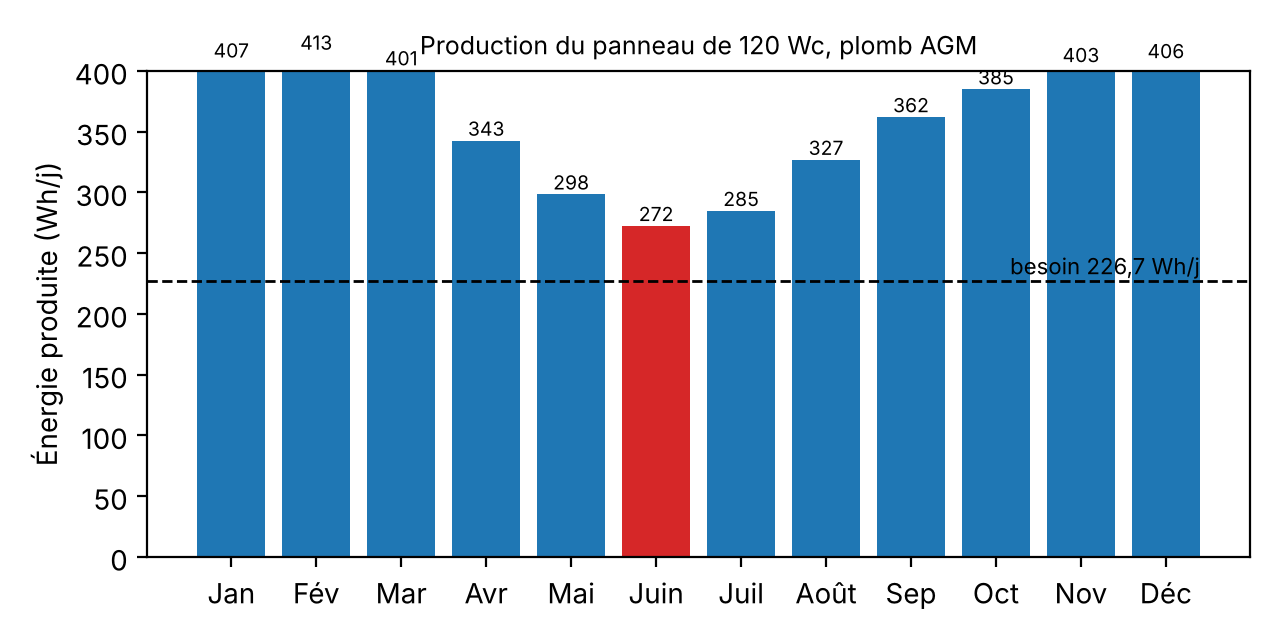
\includegraphics[width=0.78\textwidth]{img/prod_mensuelle.png}
\caption{Énergie produite chaque mois par le TE1250 (plomb AGM), comparée au besoin de \qty{226,7}{Wh/j}. Juin, le pire mois, est en rouge.}
\end{figure}

\subsubsection*{Conclusion sur le panneau}

Je peux maintenant répondre à la question de départ : le panneau fournit-il l'énergie dont la tour a besoin ? Je compare la production du pire mois au besoin journalier, puis je cherche la limite au-delà de laquelle le panneau ne suffirait plus.

\textbf{Oui, le panneau TE1250 de \qty{120}{Wc} suffit.} Le pire mois (juin), il fournit \qty{272,4}{Wh/j} avec mes batteries au plomb, pour un besoin de \qty{226,7}{Wh/j}. Il reste donc \qty{45,7}{Wh/j} de marge, soit $+20\,\%$. Cette marge sert à recharger les batteries après un jour couvert.

\naturecalc[24]{théorie (valeurs de fiches techniques et données d'ensoleillement ; rien de mesuré)}
\begin{demonstration}[limite de la conclusion]
\resultat{t_{max} \approx \qty{9,1}{h/j}}
La marge est la production moins le besoin :
\begin{align*}
\Delta E &= \qty{272,4}{Wh/j} - \qty{226,7}{Wh/j}\\
\Delta E &= \qty{45,7}{Wh/j}
\end{align*}
Je cherche la durée de marche $t_{max}$ de la pompe, en heures par jour, pour laquelle le besoin égale la production du pire mois. Le besoin hors pompe vaut \qty{97,38}{Wh/j} (électronique \qty{91,81}{Wh/j}, doseuses \qty{0,96}{Wh/j} et MPPT\ix{19} \qty{4,61}{Wh/j}). La pompe et son MOSFET\ix{15} consomment $\qty{19}{W} + \qty{0,154}{W} = \qty{19,154}{W}$ :
\begin{align*}
\qty{97,38}{Wh/j} + \qty{19,154}{W} \times t_{max} &= \qty{272,4}{Wh/j}\\
\qty{19,154}{W} \times t_{max} &= \qty{272,4}{Wh/j} - \qty{97,38}{Wh/j}\\
\qty{19,154}{W} \times t_{max} &= \qty{175,02}{Wh/j}\\
t_{max} &= \frac{\qty{175,02}{Wh/j}}{\qty{19,154}{W}}\\
t_{max} &\approx \qty{9,1}{h/j}
\end{align*}
Le planning retenu (\qty{6,75}{h/j}) est donc inférieur à cette limite.
\end{demonstration}

Cette conclusion tient à trois conditions. La pompe doit suivre le planning de l'étude (\qty{15}{min} de marche et \qty{15}{min} d'arrêt le jour, trois marches la nuit) : au-delà d'environ \qty{9}{h} de marche par jour en juin, le panneau ne suffirait plus. Le panneau doit rester propre et sans ombre. Enfin, un jour très couvert ne donne qu'environ \qty{90,6}{Wh/j} : ce jour-là, le panneau seul ne couvre pas le besoin, et ce sont les batteries qui prennent le relais (partie 5.5).

C'est une conclusion théorique : le relevé d'une journée complète (mesure M3) doit la confirmer. Le 12 novembre, j'ai seulement constaté que le panneau charge bien la batterie.

\begin{aretenir}
Pour couvrir \qty{226,7}{Wh/j} le pire mois, il faut au moins \qty{100}{Wc} avec des batteries au plomb. Le pire mois est juin, avec \qty{3,61}{kWh/m^2/j} sur un plan horizontal (Solargis). Le TE1250 de \qty{120}{Wc} fournit alors \qty{272,4}{Wh/j} en plomb AGM (\qty{304,5}{Wh/j} en LiFePO4) : marge de $+20\,\%$ ($+34\,\%$ en LiFePO4). Le panneau est suffisant ; le SLP055 seul ne l'est pas. La pompe pourrait marcher jusqu'à \qty{9,1}{h/j} en juin avant que le panneau ne suffise plus.
\end{aretenir}
\tcbset{enobox/.append style={breakable}}
